\documentclass[dvipdfmx]{jarticle}
\pagestyle{empty}
\usepackage{xcolor}
\usepackage{tikz}
\usetikzlibrary{shapes,calc,arrows.meta}
\begin{document}
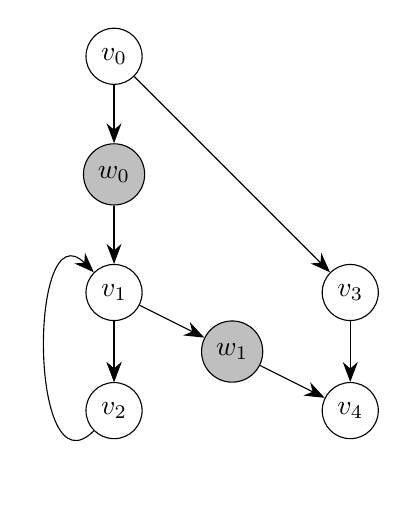
\begin{tikzpicture}
    \node[draw,circle] (V0) at (0,4.5) {$v_0$};
    \node[draw,circle,fill=lightgray] (W0) at (0,3) {$w_0$};
    \node[draw,circle] (V1) at (0,1.5) {$v_1$};
    \node[draw,circle] (V2) at (0,0) {$v_2$};
    \node[draw,circle] (V3) at (3,1.5) {$v_3$};
    \node[draw,circle,fill=lightgray] (W1) at (1.5,0.75) {$w_1$};
    \node[draw,circle] (V4) at (3,0) {$v_4$};
    \path[-{Stealth[scale=1.5]}] (V0) edge (W0) (W0) edge (V1)
    (V1) edge (V2) (V1) edge (V2) (V1) edge (W1) (W1) edge (V4)
    (V0) edge (V3) (V3) edge (V4);
    \path[-{Stealth[scale=1.5]}] (V2) [out=225,in=135,looseness=1.5] edge (V1);
\end{tikzpicture}
\end{document}